%%%%%%%%%%%%%%%%%%%%%%%%%%%%%%%%%%%%%%%%%%%%%%%%%%%%%%%%%%%%%%%%%%%%%%%%%%%%%%%%%%%%%%%%%%
\section{Evaluation}
\label{s:eval}
%%%%%%%%%%%%%%%%%%%%%%%%%%%%%%%%%%%%%%%%%%%%%%%%%%%%%%%%%%%%%%%%%%%%%%%%%%%%%%%%%%%%%%%%%%i

%
Our performance evaluation focuses on the Lobsters, WebSubmit, and HotCRP applications
from our case studies.
%
We seek to answer the four questions:
%
\begin{enumerate}[nosep]
 %
 \item Does \sys meet its security goals and provide meaningful guarantees to users?
   (\S\ref{s:eval-security})
 %
 \item How expensive are core \sys interactions, \emph{viz.}\ disguising, revealing, and
   operations over disguised data? (\S\ref{s:eval-ops})
 %
 \item How much does application latency and storage use increase when an application
   uses \sys? (\S\ref{s:eval-res})
 %
 \item How do disguise and reveal actions impact the performance of concurrently executing,
   normal application requests by other users? (\S\ref{s:eval-conc})
 %
\end{enumerate}
%
All benchmarks run on a 40-core server with Intel Xeon E5-2660 v3 CPUs and \note{XX} of RAM
running \note{Arch Linux XXX}.
%
We use the MariaDB RDMS for application data storage, but store all databases on \fn{tmpfs}
to avoid confounding factors related to persistence.
%

\subsection{Security Evaluation}
\label{s:eval-security}

%
\sys secures disguise records by encrypting them with the public key of a principal $p$.
%
The corresponding private key for $p$ is on the client device and unavailable to the
application and \sys until the client provides it as part of an operation over data
under disguise.
%
Therefore, principals who remain inactive or only perform normal application operations
that access the plaintext application DB always enjoy full privacy for their data under
disguise, as an attacker who compromises the server cannot obtain their private key.
%

%
\sys uses locators to hide which disguises the application applied to which
principals' data.
%
A disguise creates \lcapa{pd} for disguise $d$ applied to principal $p$, and links it
to the disguise's bag of ciphertexts via an index, \lcapa{pd}$\to$ bag, in \sys's
public metadata.
%
The locator itself is a random byte string and does not contain $p$ or $d$, and
only the client has knowledge of the $(p, d)$ that \lcapa{pd} corresponds to after
the disguise completes.
%
Therefore, the the state of the index contains no metadata that lets the attacker
identify $p$ or $d$.
%
While an attacker can learn that $n$ records exist for \emph{some} $p$ and $d$ by
inspecting the index and bags, they cannot identify \emph{which} $p$ or $d$.
%

%
Because \sys stores locators from disguises over pseudoprincipal-owned data as part
of its pseudoprincipal metadata, \sys's disguise composition leaks that \emph{some}
number of disguises have applied to pseudoprincipal $q$.
%
However, these locators are encrypted with $q$'s private key, which is only accessible
by decrypting a bag protected by another principal's private key, a chain that extends
back to some natural principal $p$.
%
This prevents an attacker from finding out which bags belong to $q$, and therefore
also hides which bags correspond to natural principals' data.
%
Because $q$ is dissociated from the natural principal $p$ that speaks for $q$
(possibly via intermediate principals), the attacker cannot determine if natural
principal $p$ ever existed, nor if they have any data in \sys.
%

%
If an attacker compromises the server at time $t$, they can harvest any private key
that a client provides for operations after $t$.
%
The attacker can therefore reveal all current data under disguise stored in \sys and
encrypted with this private key.
%
Likewise, when a client provides $(\lcapa{pd}, p, d)$ to operate over data under disguise,
the attacker learns the correspondence between \lcapa{pd} and $(p, d)$.
%
But this merely makes the attack more efficient, as the attacker can already discover
$p$'s disguise history by attempting to decrypt all bags with $p$'s private key.
%
However, provided that the application deletes ciphertexts from \sys after revealing
the data, the attacker cannot gain access to any previously-revealed data that users
subsequently deleted from the application database.
%
\sys makes no guarantees for users who actively use data under disguise after
compromise, but always protects inactive users.
%

%
After a compromise occurs and is detected, users who performed operations on data
under disguise and whose private keys might have been compromised must start using new
keys.
%
This is easy: the application tells the client to generate a new key pair, and then
calls \fn{RegisterPrincipal} to register the natural principal's new public key with
\sys.
%
Future disguises now use this public key; \sys could also re-encrypt existing data
under disguise, but our prototype does not do so, as this data is already potentially
compromised.
%
A conscientious user might change their keypair for the application on a regular basis
to protect their data against undetected compromises.
%

\subsection{Performance of \sys Operations}
\label{s:eval-ops}

%
Next, we measure \sys's performance using disguises from our three case study
applications: WebSubmit, Lobsters, and HotCRP.
%
For each application, we measure the latency of normal operations as well as
privacy transformations.
%
In order to measure the extra cost added by \sys's cryptographic operations,
we implemented a manual, irreversible version of each privacy transformation,
as a developer would, by directly modifying the application database, and
measure its latency.
%
\sys allows applications to provide additional functionality, such as account
restoration and editing data under disguise, and we measure the latency of these
operations too.
%
A good result for \sys would show no overhead on normal application operations,
competitive performance with manual privacy transformations, and reasonable
latencies for data-revealing operations (\eg a few seconds for account
restoration).
%

\begin{figure}[t]
    \centering
    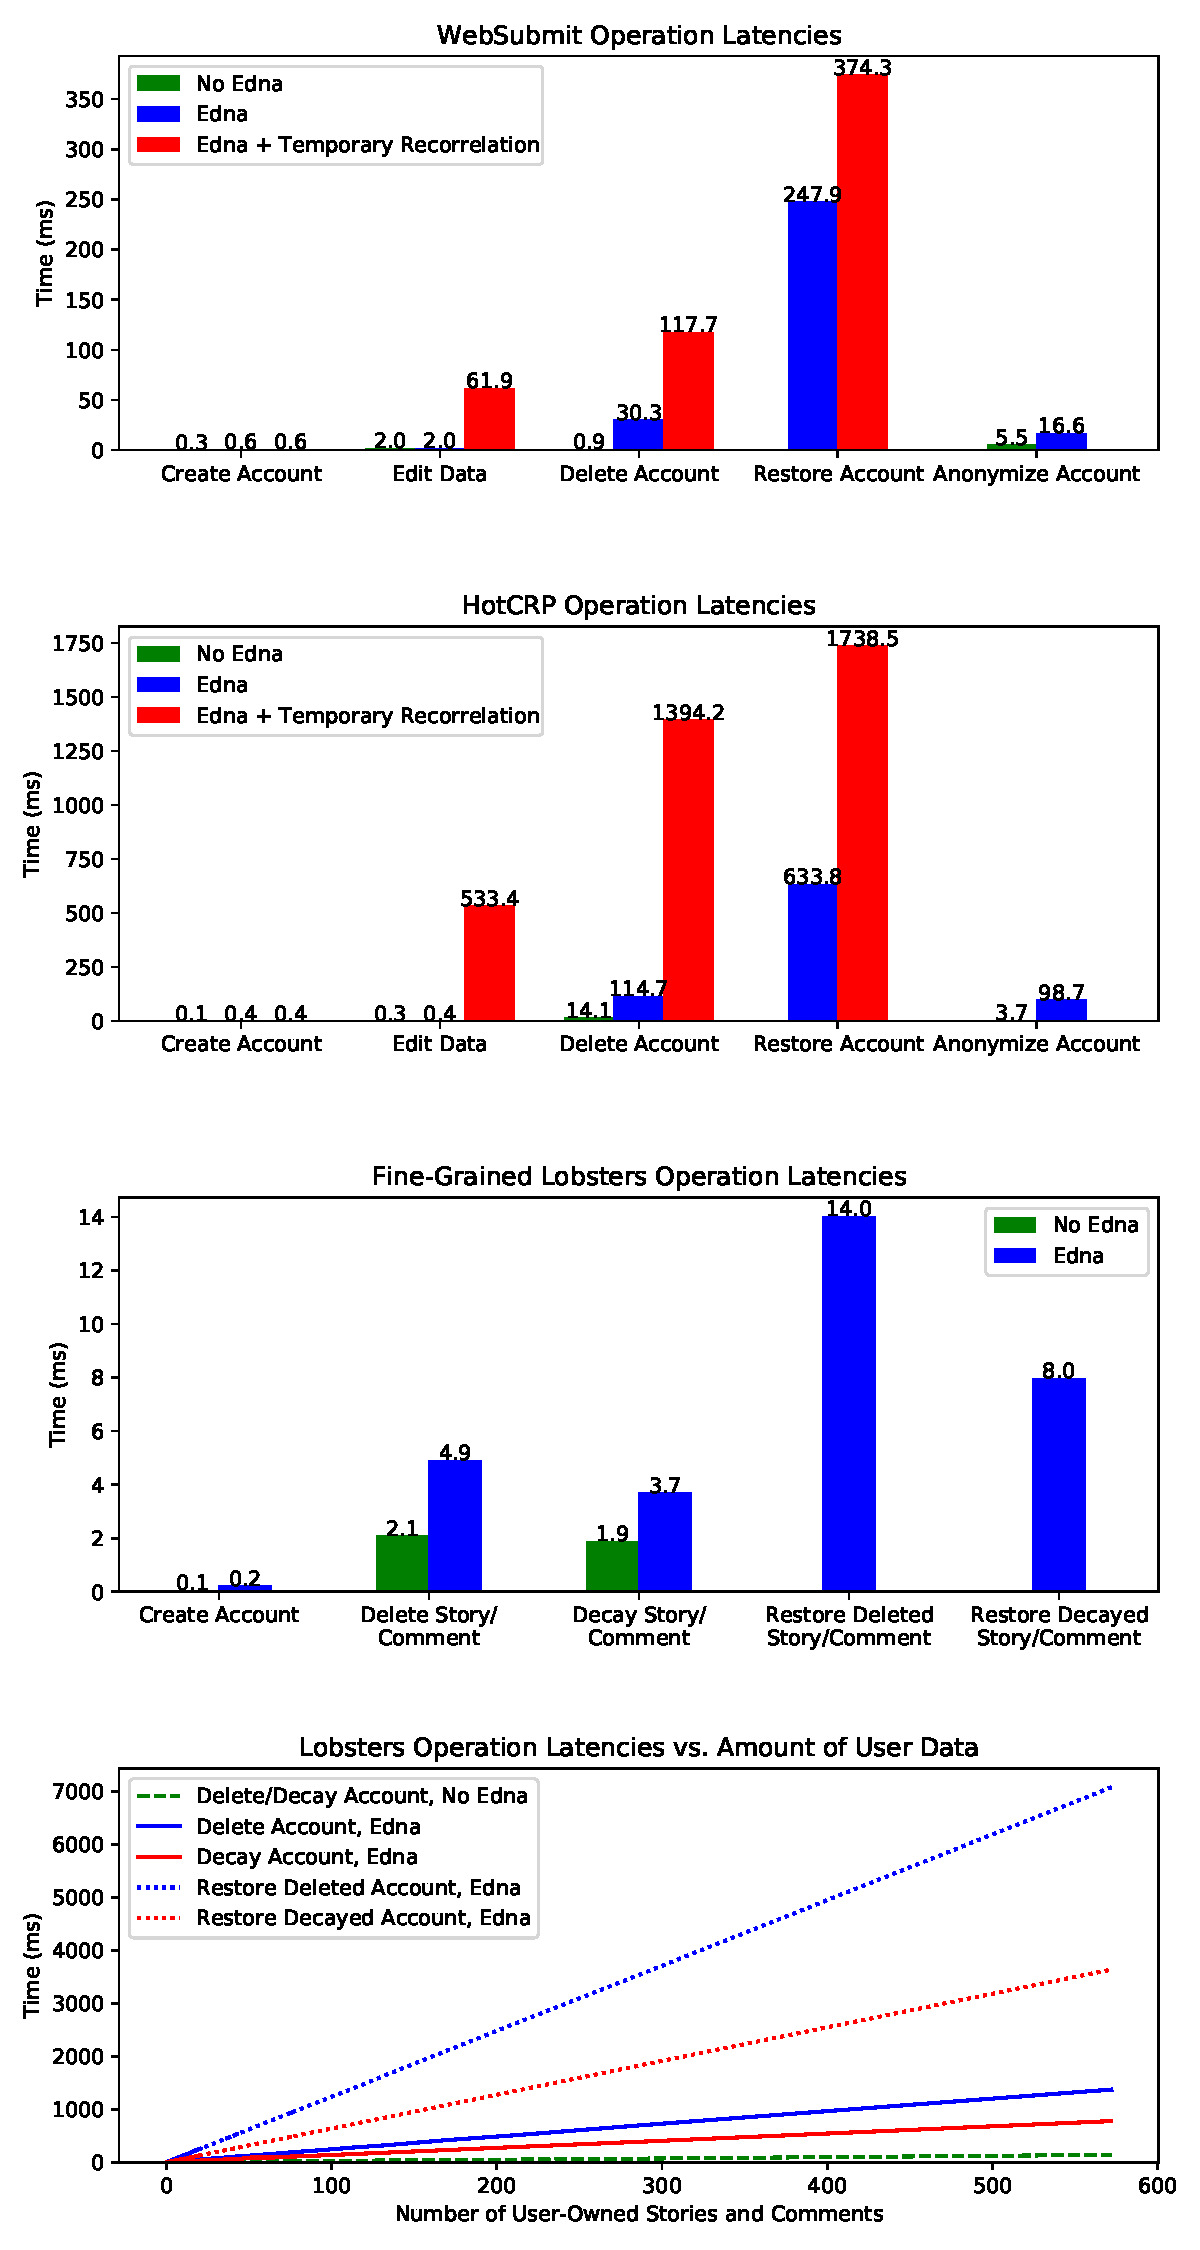
\includegraphics[width=0.5\textwidth]{figs/client_op_stats}
    \caption{Latencies of disguise-related actions when implemented manually by the
    application developer without \sys, and with \sys.
    Each bar shows the median latency; ranges indicate the 5th to 95th
    percentile latencies.}
    \label{fig:client_opstats}
\end{figure}

\begin{table*}[h!]
\begin{center}
\begin{tabular}{ c c }
\textbf{DB Op} & \textbf{Time (ms)}\\
\hline
Update DB Row & 0.1\\
Select DB Rows & 0.2\\
Remove DB Rows & 0.2\\
Reveal Deleted Row (DB Select + Insert) & 0.2 \\
Create + Register Principal & 0.1\\
\end{tabular}
\quad
\begin{tabular}{ c c }
\textbf{Crypto Op} & \textbf{Time (ms)}\\
\hline
Generate Keypair & 301\\
Encrypt SpeaksFor Record & 0.4\\
Decrypt SpeaksFor Record & 3.0\\
Encrypt Diff Record & 0.3\\
Decrypt Diff Record & 3.0\\
\end{tabular}
\end{center}
\caption{Amount of time required to run different operations required to apply and reveal disguises.}
\label{tab:opstats}
\end{table*}

\paragraph{WebSubmit.}
%
We run WebSubmit benchmarks with a database seeded with 2,000 users, 20
lectures with four questions each, and an answer for each question for
each user (160k total answers).
%
This might correspond to all classes in a department, or to a large AI class.
%
We measure end-to-end latency, which includes request processing in WebSubmit,
\sys's operations, and the response to the client.
%
The amount of data under disguise is constant across users, so we would expect
low variance in the results.
%

%
Figure~\ref{fig:websubmit-ops} shows the median latency for two normal operations
(creating an account and editing unanonymized data), two disguises (delete account
and anonymizing an account), and two operations over data under disguise (editing
anonymized data and restoring the account).
%
Normal operations have comparable latencies with and without \sys.
%

%
\sys's disguise-based account deletion takes 2.9ms, \vs 0.9ms in the manual
baseline.
%
This makes sense, as \sys encrypts database diffs and speaks-for records, while
the baseline only deletes data from the application DB.
%
The difference is greater for account anonymization, where \sys takes 10.8ms,
while the baseline takes less than 0.1ms.
\ms{why?}
%
Finally, \sys enables operations over data under disguise, which are impossible in
the baseline; these take 10.2ms and 21ms, well within acceptable interactive
latencies for web applications.
%
The simplicity of WebSubmit's disguises---which touch at maximum two database
tables---lead to fairly low latencies even for involved operations such as
restoring a deleted account (21ms).
%

\paragraph{HotCRP.}
%
We run the HotCRP experiments on a database seeded with 450 total users (50 of
whom are PC members), 450 papers, and four reviews and four comments per paper,
distributed evenly among PC members.
%
The benchmark measures the server-side latency to perform disguising and
application operations.
%
HotCRP supports the same disguise-related operations as WebSubmit.
%

HotCRP reviewers have slightly more variable amounts of data \lyt{TODO?} depending on the
assignment of papers to reviewers. HotCRP's disguises are far more complex than
WebSubmit's, touching 12 tables, and performing a mix of deletions and
decorrelations, leading to higher median latencies in general, even for the baseline.


\paragraph{Lobsters.}
%
We run Lobsters benchmarks on a database seeded with 14.5k users, which
is the late-2021 size of the real Lobsters site.
%
These users have \note{40k} stories, and \note{120k} comments with votes;
stories, comments, and votes are distributed among users according to
statistics from the actual Lobsters deployment~\cite{lobsters-data}.
%
The benchmark measures server-side latency of disguising and application
operations.
%

Lobsters supports account creation and deletion/restoration as well, but has account decay (and
subsequent restoration) instead of account anonymization.  It does not support editing anonymized
data (accounts can be restored in order to edit decorrelated data). In these benchmarks, we measure
the cost of GDPR-compliant account deletion and restoration.


Lobsters users' amount of data follows a skewed distribution, with most of the 5000 users
having fewer than 10 stories and comments, and a handful of users having over 300 stories and
comments. Lobster supports more complex disguises than WebSubmit and HotCRP,
touching 15 tables, and performing a mix of deletions, decorrelations, and modifications. This leads
to a higher latency as the amount of user data grows comparable to that of users in HotCRP and
WebSubmit.

\paragraph{Drill-Down.}
%
Latency-critical tasks such as editing (unanonymized) data or
creating an account are largely unaffected by \sys.
%
To explain these costs, we break them down into fine-grained operations shown in
Table~\ref{tab:opstats}: every disguise action requires some DB operations and,
if using \sys, may require cryptographic operations.

\textbf{Creating an account} with or without \sys performs a database insert. Using \sys additionally
requires registering the new user as a principal, which assigns the user a (pre-generated)
private-public key pair, stores metadata about the new principal's key in \sys's storage, and
returns the corresponding private key to the application.
Using \sys thus incurs only the cost of an extra database operation, since the high cost of key
generation is taken offline.

\textbf{Editing data} with or without \sys simply performs database updates. Editing anonymized
data, however, requires \sys to decrypt (with the client-provided decryption capability) \emph{all}
speaks-for records at the client-provided locator until it finds a speaks-for record linking the
client to the currently-owning pseudoprincipal.  For example, if anonymization of a user account
generates 20 speaks-for record ciphertexts at the same locator, then editing anonymized data may
perform up to 20 decryptions to determine which pseudoprincipals the client can act for.  Record
batching drastically decreases this cost by performing only one decryption to decrypt all speaks-for
records for a particular client and disguise.

\textbf{Account deletion or data decay} with or without \sys performs the same database operations
to remove, modify, or anonymize data. \sys incurs increased costs by additionally encrypting and
inserting one diff record for each deleted or modified object, and one speaks-for record for each
anonymized object.  With record batching, encryption occurs once per account, rather than once per
object.

\textbf{Account restoration} is only possible with \sys. \sys decrypts a record for each
piece of modified/removed/anonymized data, and performs database checks to ensure the data can be restored
(\eg that the corresponding lecture of an answer to reinsert still exists). If the checks pass
(which they do in this benchmark), \sys restores the data stored in the diffs.
Record batching drastically decreases this cost by performing only one decryption to decrypt all
records to restore.

\textbf{Anonymization} with or without \sys generates one pseudoprincipal per object to anonymize
(\eg answers for lectures in WebSubmit, or reviews in HotCRP). Anonymization selects the relevant answers
to anonymize, generates new pseudoprincipals, and performs DB queries to insert new pseudoprincipals
and to update objects to point to these new pseudopricipals (\eg updating foreign keys).
\sys incurs increased costs by additionally generating per-pseudoprincipal speaks-for records, and
encrypting and storing these speaks-for records with the appropriate public keys.
With record batching, encryption occurs once per account, rather than once per object.

\begin{figure}[t]
    \centering
    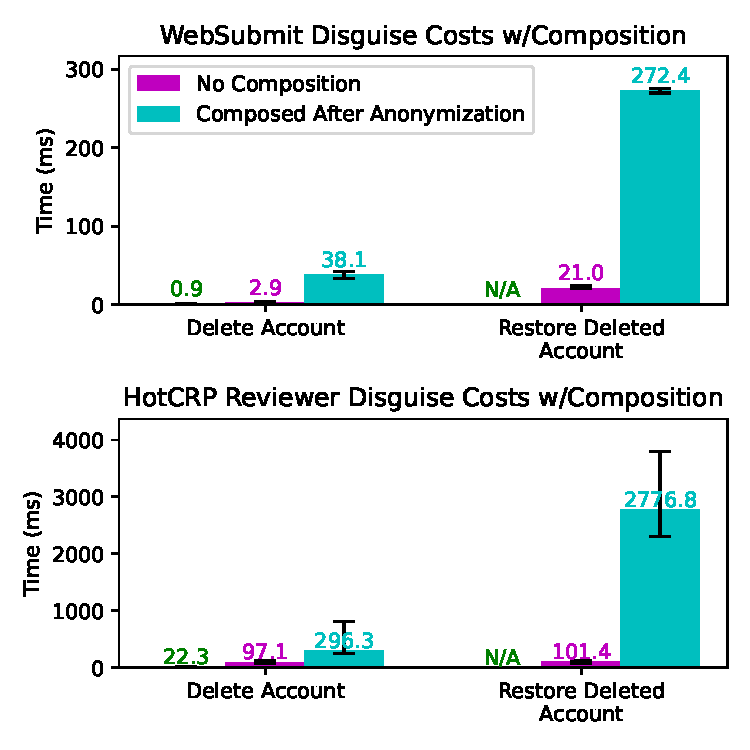
\includegraphics[width=0.45\textwidth]{figs/composition_stats}
    \caption{Latency of account delete and restore before anonymization vs. composed after anonymization.}
    \label{f:composition}
\end{figure}

\begin{figure*}[t]
    \centering
        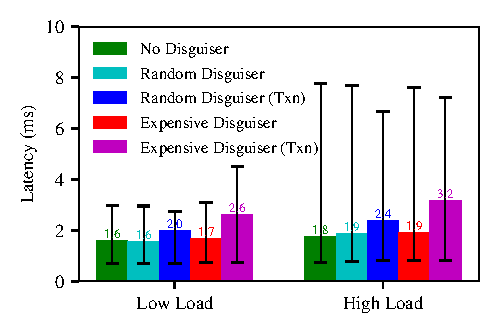
\includegraphics[width=0.45\textwidth]{figs/lobsters_concurrent_results}
        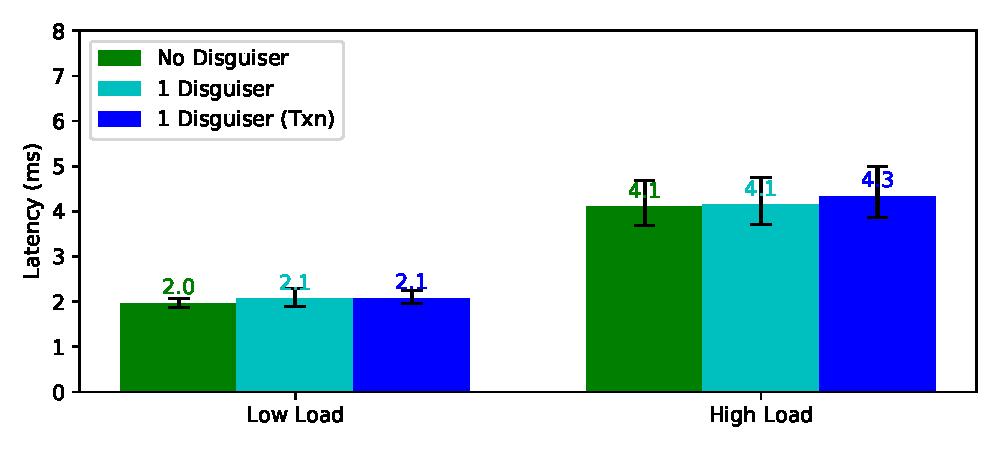
\includegraphics[width=0.45\textwidth]{figs/websubmit_concurrent_results}
    \caption{Impact of continuously applying and revealing account deletion disguises (non-transactional and transactional) on users concurrently running
    normal application operations. We show the median latency; ranges indicate the 5th to 95th
    percentile latencies.
    \textbf{Left (Lobsters)} tests the normal Lobsters traffic in the presence of an expensive
    disguiser (owning >6000 data objects) and a cheap disguiser (ownering <10 data objects). Even an expensive disguiser has minimal impact when user load is low; however, the impact increases as the server load increases, and if the
    disguise is transactional.
    \textbf{Right (WebSubmit)} tests an adversarial, write-only user workload of edits that
    modify the same table. All users have approximately the same amount of data (4 answers for 20
    lectures), and one user is chosen to continuously delete and restore their account. Here,
    disguising has minimal impact on latency even at high load.
    }
    \label{fig:concurrent}
\end{figure*}

\textbf{Composing Deletion After Anonymization.}
\lyt{TODO}
Account deletion post-anonymization requires \sys to perform temporary recorrelation find data of
pseudoprincipals that the user is authorized to remove along with their account. \sys incurs latency
increases from decrypting all speaks-for records of the user, and from performing the deletion or
modification queries for each discovered pseudoprincipal (in addition to the original user).

Account restoration may also restore pseudoprincipal-associated data, which requires temporary
recorrelation to access to pseudoprincipal-associated records produced from the account deletion.
\sys thus additionally decrypt speaks-for records for all pseudoprincipals of the user, which causes
the the increase in latency.\lyt{Numbers?}

%%%%%%%%%%%%%%%%%%%%%%%%%%%%%%%%%%%%%%%%%%%%%%%%%%%%%%%%%%%%%%%%%%%%%%%%
\subsection{Resource Use}
\label{s:eval-res}

Each generated pseudoprincipal adds an additional row to the users table in WebSubmit; \sys also
stores public-key metadata for each principal (and pseudoprincipal), and (in-memory) encrypted
ciphertexts for records.  Clients keep track of capabilities and locators that are emailed to them in
the form of URLs that allow for account restoration or post-anonymization editing.

%%%%%%%%%%%%%%%%%%%%%%%%%%%%%%%%%%%%%%%%%%%%%%%%%%%%%%%%%%%%%%%%%%%%%%%%
\subsection{Impact on Normal Application Use}
\label{s:eval-conc}

Figure~\ref{fig:concurrent} shows the impact of concurrently-running disguise actions on the latency
of normal application operations.

We first test the impact of disguising in Lobsters. We first achieve ~80\% CPU load by running
30 threads that model production Lobsters traffic. These threads simulate performing different
Lobsters operations (\eg loading the front-page, posting stories) according to measured access
frequencies and popularity distributions in production\lyt{CITE}. In this workload, 85\% of all
operations are front-page loads, which fetching stories and vote counts.

An additional number of threads simulate disguising users: these users (in the worst-case) decide to
simultaneously delete their account (\eg in response to some social media campaign). At some later
point in time, these users decide to come back and (in the worst case) simultaneously restore their
accounts.
We observe that even when the number of disguisers increases to 100, the latency of normal Lobsters
operation remains unaffected.

We then test an adversarial, write-only workload with WebSubmit. As a baseline, we achieve ~60\% CPU
load by running 100 threads that each continuously edit a user's lecture answers with 250-500ms
pauses between edits. This write-heavy workload achieves particularly high contention because all
edit queries modify the same database table; MySQL uses table-level locking for \texttt{MEMORY}
tables.

We then add an additional number of threads to simulate simultaneously disguising users.  While
fewer than 16 users disguising themselves at once has minimal impact on edit latency, 30 users doing
so causes spikes up to 4000ms.  These spikes come in pairs, with the larger second spike in the pair
coinciding with concurrent revealing (and the first of the pair coinciding with disguising);
revealing has greater impact due to its higher latency and compute costs.
%
Record batching improves these results by reducing the load generated by disguise actions: latency
spikes decrease to under 1500ms.

While we focus on normal application operation latency, we note that
disguise operation latency increases proportional to the overall system load (\eg due to MySQL’s
table-level locking). But this is acceptable, as disguises aren't time critical; in practice, they
still complete within a few seconds even at 60-80\% system load.
%
What matters is that normal application requests have acceptably low latency even in the presence of
disguising, which we achieve under realistic workloads (largely reads, with queries dispersed among
tables). If the workload becomes adversarial, \sys can prevent normal operation latency spikes by
rate-limiting disguise actions.
